\subsection{Reconstruction des jets}\label{chapter-CMS-section-jets_reco}
La phénoménologie des jets est présentée dans le chapitre~\refChMSSM.
Les partons, \ie\ les quarks et les gluons, ne peuvent pas être directement observés dans le détecteur.
Leur signature expérimentale est un jet, \ie\ un flux collimé de particules stables composé de hadrons, de leptons et de photons.
Afin de pouvoir étudier le processus initial dont sont issus les partons à l'origine des jets observés, il est nécessaire de reconstruire ces jets en regroupant l'ensemble des particules les constituant.
\par
À partir des particules identifiées à l'aide de l'algorithme de \emph{Particle Flow} (\PF), un regroupement de celles-ci permet d'obtenir la liste des jets de l'événement.
Il existe plusieurs algorithmes de regroupement dont le principe est décrit dans la section suivante.
\par
Les jets identifiés selon la procédure présentée ci-après sont par la suite calibrés en énergie.
Cette calibration est l'objet du chapitre~\refChJERC.
\subsubsection{Algorithmes de regroupement}\label{chapter-CMS-section-jets_reco-subsec-algo}
Il existe deux catégories d'algorithmes permettant de regrouper les particules en jets, les algorithmes de cônes et ceux de recombinaison séquentielle.
Les émissions de partons sont plus importantes pour les basses énergies (limite infrarouge) ou lorsqu'un parton émis de façon colinéaire au parton initial (limite colinéaire), comme discuté dans le chapitre~\refChMSSM.
Afin de rendre compte de ce comportement de QCD, les algorithmes de regroupement doivent être insensibles à l'ajout d'une particule de basse énergie ou au partage d'une particule en deux autres d'énergies inférieures. C'est ce que l'on appelle l'insensibilité IRC, pour \emph{InfraRed and Colinear}.
La plupart des algorithmes de cônes ne sont pas IRC-insensibles, alors que la majorité des algorithmes de recombinaison séquentielle le sont.
\begin{wrapfigure}{R}{.45\textwidth}
\centering
\begin{tikzpicture}[scale=1.5]
\clip (-.25, -.25) rectangle (2,2);

\draw [thick, -latex] (0,0) --+ (45:2) node [above right] {$\vec{a}$};
\draw [thick, ltcolorgreen, -latex] (0,0) --+ (40:2) node [right] {$\vec{p}_1$};
\draw [thick, ltcolorred, -latex] (0,0) --+ (60:2) node [left] {$\vec{p}_2$};

{\color{ltcolorblue}
\printDR{0.4}{45}
\draw (30:.75) node [right] {$R_c$};
}
\end{tikzpicture}
\caption[Regroupement par algorithme de cônes.]{Regroupement par algorithme de cônes. La particule de direction $\vec{p}_1$ est ajoutée au cône, celle de direction $\vec{p}_2$ ne l'est pas.}
\label{fig-schema_algo_cones}
\end{wrapfigure}
\paragraph{Les algorithmes de cônes} regroupent toutes les particules ayant une direction $\vec{p}$ telle que la distance $\Delta R_{pa}$ à la direction de l'axe du cône $\vec{a}$ dans le plan $(\eta,\phi)$ est inférieure à une distance de coupure $R_c$, comme illustré sur la figure~\ref{fig-schema_algo_cones}, \ie\ si
\begin{equation}
\Delta R_{pa} ^2 = (\eta_p - \eta_a)^2 + (\phi_p - \phi_a)^2 < R_c^2
\mend
\end{equation}
Alors, la direction $\vec{a}$ du cône est redéfinie comme étant la direction moyenne de toutes les particules rassemblées dans ce cône. Ce processus est itéré jusqu'à la stabilisation des cônes.
Enfin, une particule ne pouvant appartenir qu'à un seul jet, les cônes sont séparés en cas de superposition.
\par L'algorithme \emph{Seedless Infrared Safe Cone} ou \textsc{SISCone}~\cite{SISCone} est un exemple d'algorithme de cônes IRC-insensible.
Dans un premier temps, tous les cônes stables possibles sont construits.
Ces cônes sont alors fusionnés, les cônes ayant l'impulsion transverse la plus grande absorbant des cônes d'impulsion transverse moindre dont ils contiennent déjà une fraction des constituants.
Un exemple de reconstruction de jets à l'aide de l'algorithme \textsc{SISCone} est présenté sur la figure~\ref{fig-chapter-CMS-section-jets_reco-subsec-algo-examples}.
\begin{figure}[b]
\centering
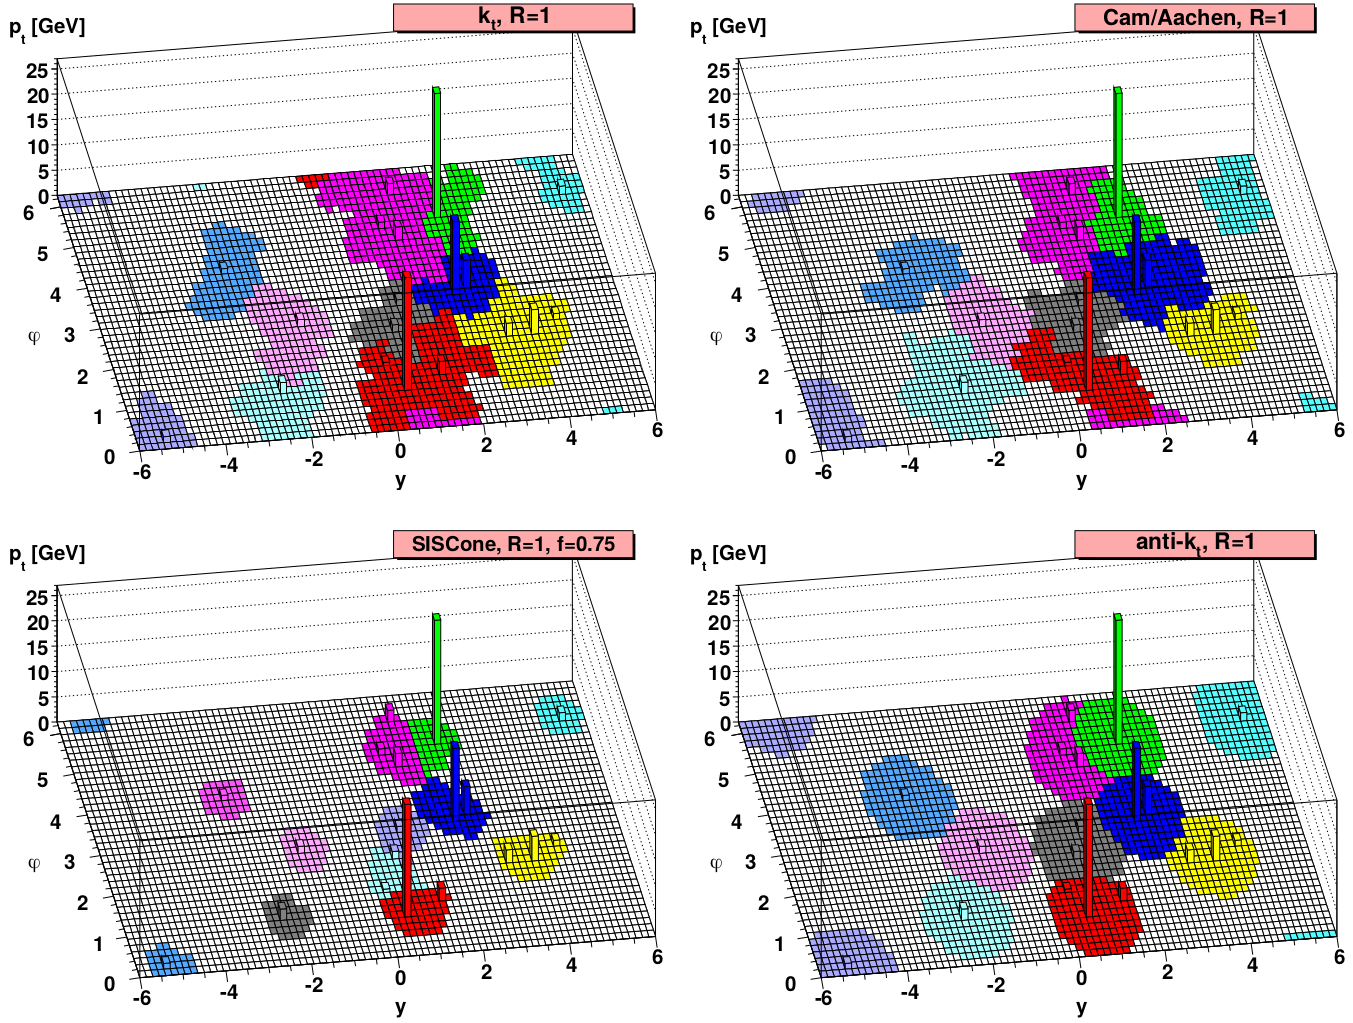
\includegraphics[width=.8\textwidth]{\PhDthesisdir/plots_and_images/from_Cacciari_antikT/forme_des_jets.png}
\caption[Formes des jets reconstruits à partir de différents algorithmes.]{Formes des jets reconstruits à partir de différents algorithmes pour un même événement~\cite{Cacciari_antikT}. En haut à gauche, \kT; en haut à droite, C/A; en bas à gauche, \textsc{SISCone}; en bas à droite, anti-\kT. L'algorithme anti-\kT\ permet d'obtenir des jets de forme régulière.}
\label{fig-chapter-CMS-section-jets_reco-subsec-algo-examples}
\end{figure}
\paragraph{Les algorithmes de recombinaison séquentielle} commencent par considérer que chaque particule forme un pseudo-jet d'une seule particule~\cite{Cacciari:2011ma}.
Puis, de manière itérative et à l'aide d'une métrique donnée, la paire composée des deux jets les plus proches fusionne tant que la distance entre eux est en-deçà d'une valeur seuil. Les jets fusionnés donnent la liste des jets de l'événement. Il est également possible de fixer le nombre de jets à déterminer et non la valeur seuil de la distance entre les jets à fusionner.
\par Plusieurs métriques de distance peuvent être définies, chacune correspondant à un algorithme de recombinaison séquentielle proposant des regroupements différents.
\begin{description}
%\item[Algorithme de Durham~\cite{???}] La distance $d_{ij}$ entre deux jets $i$ et $j$ est
%\begin{equation}
%d_{ij} = 2 \, \min(E_i^2, E_j^2) \, \frac{1-\cos\theta_{ij}}{Q^2}
%\end{equation}
%où $E_x$ est l'énergie du jet $x$, $\theta_{ij}$ l'angle entre les directions des deux jets et $Q$ l'énergie dans le centre de masse de la collision.
%Cet algorithme a l'avantage de regrouper les particules très fidèlement vis-à-vis de la gerbe partonique, mais les jets obtenus possèdent une géométrie spatiale irrégulière, comme cela se voit sur la figure~\ref{fig-chapter-CMS-section-jets_reco-subsec-algo-examples}.
\item[Algorithme \kT~\cite{Catani_kT_algo}] La distance $d_{ij}$ entre deux jets $i$ et $j$ est définie par
\begin{equation}
d_{ij} = \min({\pT}_i^2, {\pT}_j^2) \, \frac{\Delta R_{ij}^2}{R^2}
\mend[,]
\end{equation}
où
\begin{equation}
\Delta R_{ij}^2 = (\eta_i-\eta_j)^2 + (\phi_i-\phi_j)^2
\label{eq-DRij_jets_def}
\end{equation}
avec $\eta_x$ la pseudo-rapidité,
$\phi_x$ l'angle azimutal et
${\pT}_x$ l'impulsion transverse du jet $x$ et
$R$ un paramètre libre.
Cet algorithme a l'avantage de regrouper les particules très fidèlement vis-à-vis de la gerbe partonique, mais les jets obtenus possèdent une géométrie spatiale irrégulière, comme cela se voit sur la figure~\ref{fig-chapter-CMS-section-jets_reco-subsec-algo-examples}.
\item[Algorithme de Cambridge/Aachen~\cite{Dokshitzer_1997,wobisch1999hadronization}] La distance $d_{ij}$ entre deux jets $i$ et $j$ est définie par
\begin{equation}
d_{ij} = \frac{\Delta R_{ij}^2}{R^2}
\mend[,]
\end{equation}
où $\Delta R_{ij}^2$ est défini par l'équation~\eqref{eq-DRij_jets_def}
et $R$ est un paramètre libre. Le regroupement des jets est ainsi uniquement basé sur l'écart angulaire.
\item[Algorithme anti-\kT~\cite{Cacciari_antikT}] La distance $d_{ij}$ entre deux jets $i$ et $j$ est définie par
\begin{equation}
d_{ij} = \min\left(\frac{1}{{\pT}_i^2}, \frac{1}{{\pT}_j^2}\right) \, \frac{\Delta R_{ij}^2}{R^2}
\mend[,]
\end{equation}
où $\Delta R_{ij}^2$ est défini par l'équation~\eqref{eq-DRij_jets_def},
${\pT}_x$ l'impulsion transverse du jet $x$ et $R$ un paramètre libre.
Le regroupement des particules se fait ainsi autour de celles de plus hautes énergies.
Cet algorithme propose un regroupement des particules moins fidèle à la gerbe partonique, mais produit des jets de forme régulière, comme cela se voit sur la figure~\ref{fig-chapter-CMS-section-jets_reco-subsec-algo-examples}.
\end{description}
\par Le temps de calcul de ces algorithmes est un enjeu majeur au LHC.
Leurs temps d'exécutions sont représentés en fonction du nombre d'interactions d'empilement sur la figure~\ref{fig-chapter-CMS-section-jets_reco-subsec-algo-perfs}.
Les algorithmes de Cambridge/Aachen, \kT\ et anti-\kT\ sont les plus rapides, ils permettent le traitement d'un événement en moins d'une milliseconde dans les conditions des collisions proton-proton du LHC.
Les jets de formes plus régulières sont obtenus avec anti-\kT.
C'est cet algorithme de regroupement qui est utilisé dans le cadre de l'expérience CMS.
Sur la figure~\ref{fig-Jet_PF_Composition_RunII} sont illustrées les compositions des jets reconstruits lors des trois années du Run~II. L'écart entre données réelles et simulées n'excède généralement pas \SI{2}{\%}.
\begin{figure}[h]
\centering
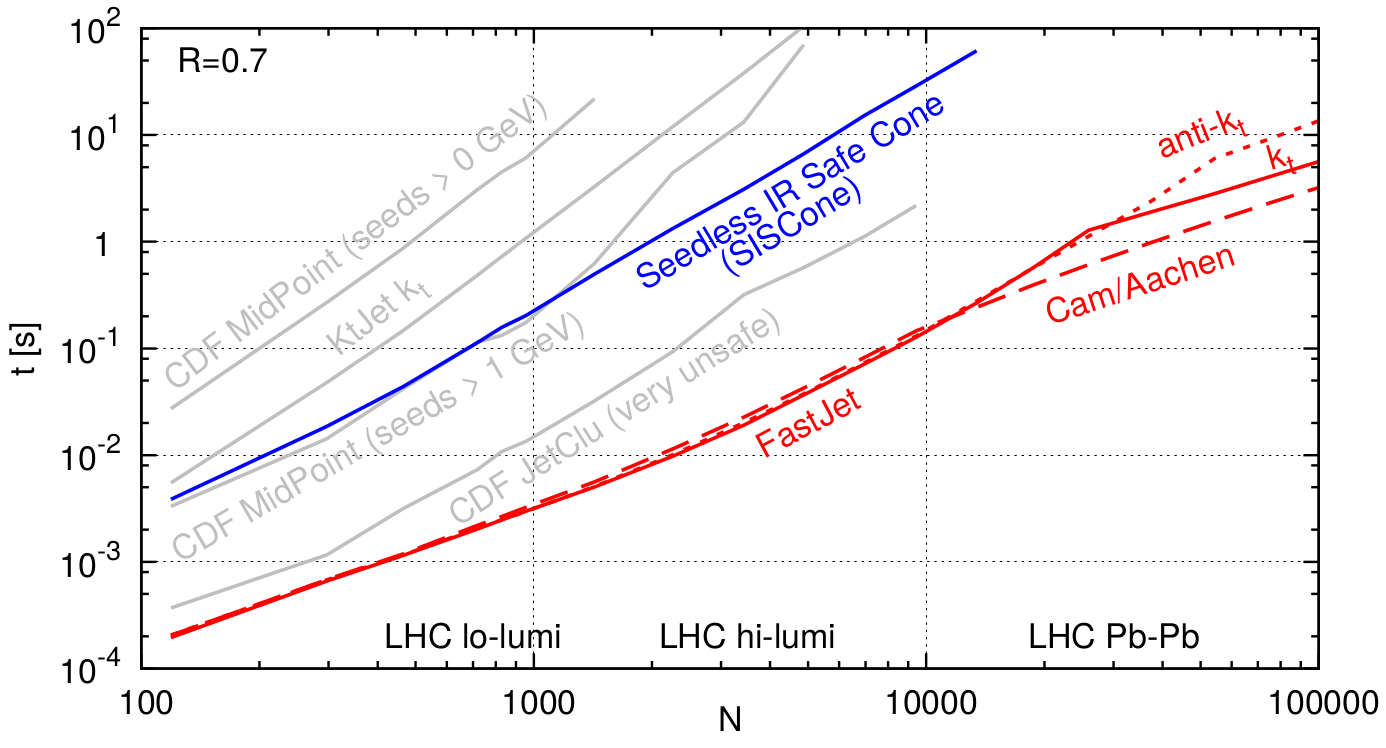
\includegraphics[width=.7\textwidth]{\PhDthesisdir/plots_and_images/from_towards_jetography/temps_de_calcul.png}
\caption[Temps de recombinaison d'un événement dijet.]{Temps de recombinaison d'un événement dijet simulé de \SI{50}{\GeV} contenant $N$ interactions d'empilement pour différents algorithmes de reconstruction des jets~\cite{towards_jetography}.}
\label{fig-chapter-CMS-section-jets_reco-subsec-algo-perfs}
\end{figure}
\begin{figure}[h]
\centering
\subcaptionbox{Année 2016.\label{subfig-Jet_PF_Composition_2016}}[.3\textwidth]
{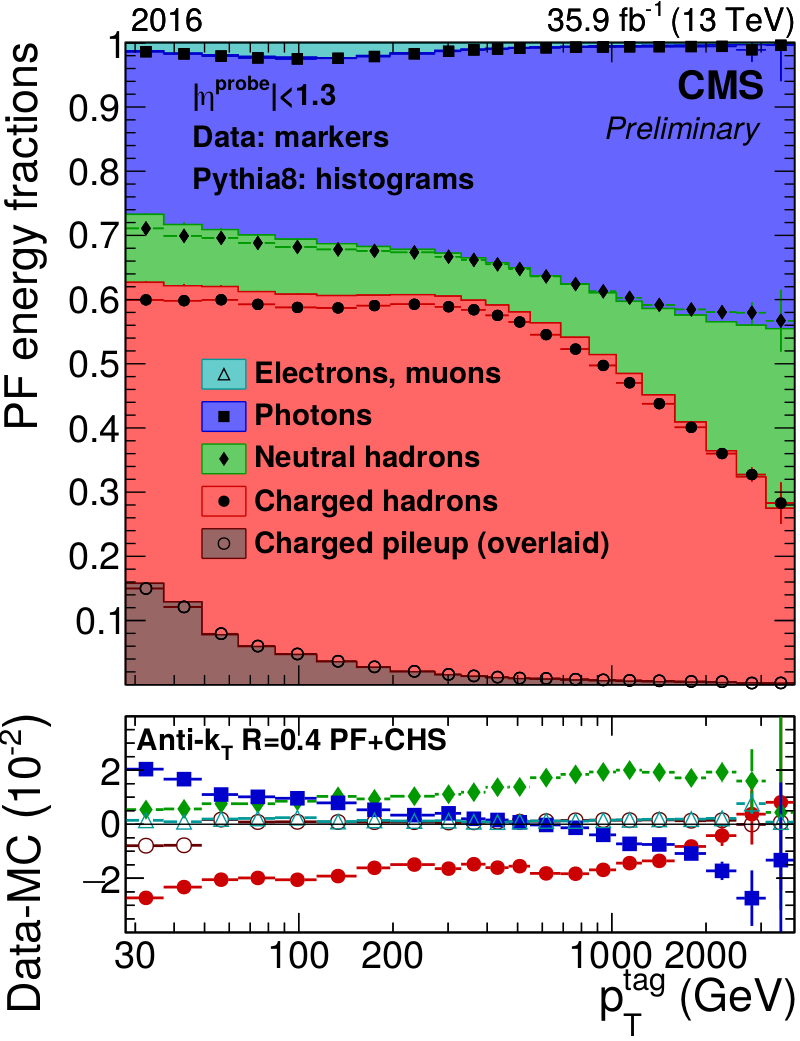
\includegraphics[width=.3\textwidth]{\PhDthesisdir/plots_and_images/from_CMS-DP-2020-019/Jet_PF_Composition_2016.png}}
\hfill
\subcaptionbox{Année 2017.\label{subfig-Jet_PF_Composition_2017}}[.3\textwidth]
{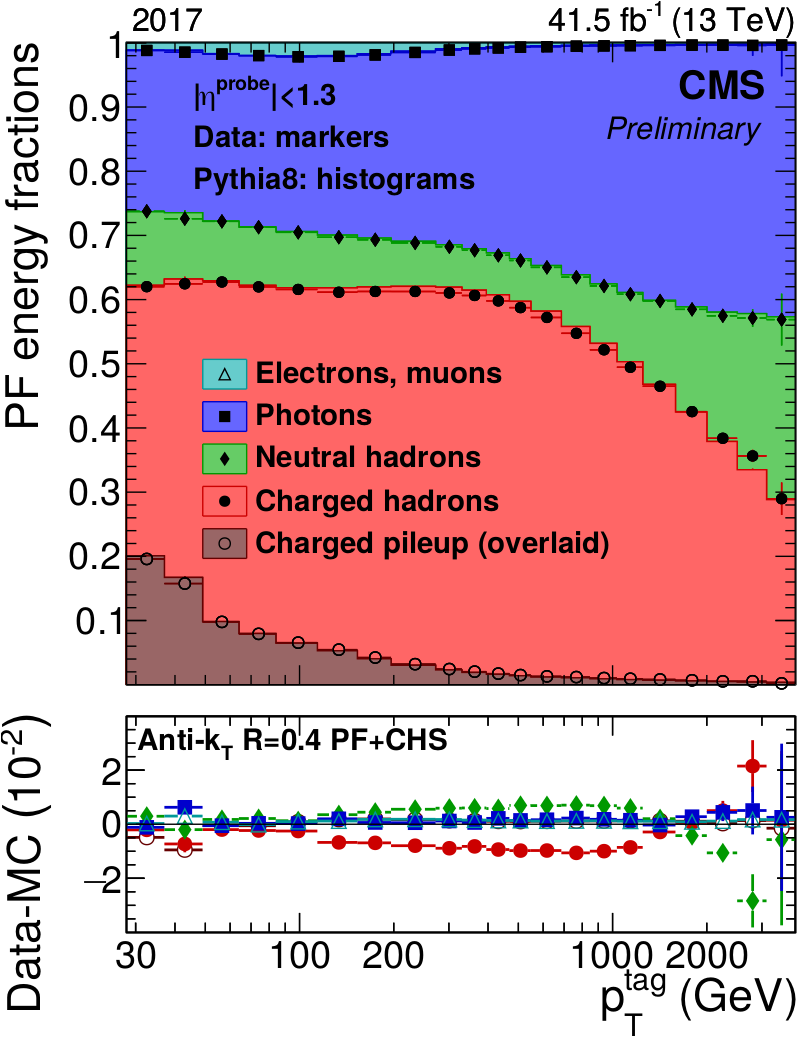
\includegraphics[width=.3\textwidth]{\PhDthesisdir/plots_and_images/from_CMS-DP-2020-019/Jet_PF_Composition_2017.png}}
\hfill
\subcaptionbox{Année 2018.\label{subfig-Jet_PF_Composition_2018}}[.3\textwidth]
{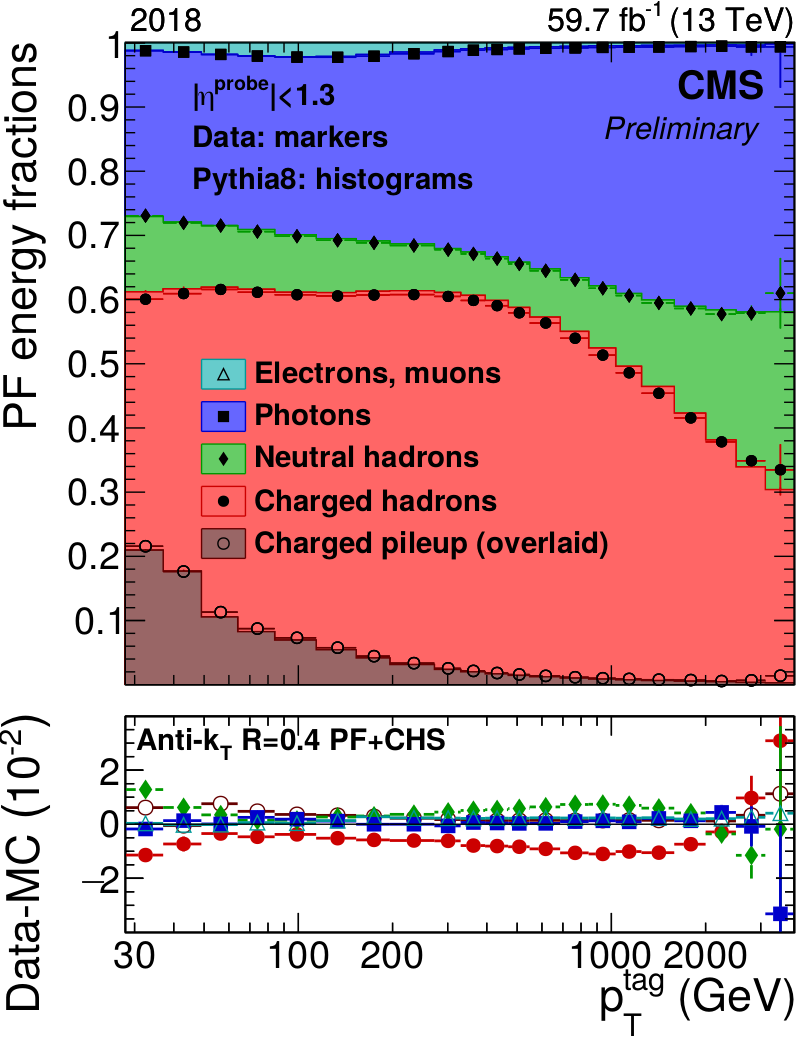
\includegraphics[width=.3\textwidth]{\PhDthesisdir/plots_and_images/from_CMS-DP-2020-019/Jet_PF_Composition_2018.png}}
\caption[Compositions des jets reconstruits lors du Run~II.]{Composition des jets reconstruits à l'aide de l'algorithme anti-\kT\ lors du Run~II~\cite{CMS-DP-2020-019} en fonction de l'impulsion transverse du jet dans les données réelles (Data, histogrammes avec des points) et simulées (MC, histogrammes en couleurs). La partie \emph{Charged pileup (overlaid)} en brun correspond à la fraction du jet retirée par la procédure CHS décrite dans le chapitre~\refChJERC.}
\label{fig-Jet_PF_Composition_RunII}
\end{figure}
\subsubsection{Identification des jets dans CMS}\label{chapter-CMS-section-jets_reco-subsec-jetID}
Les jets ainsi reconstruits à l'aide des algorithmes de recombinaison sont en réalité des \og candidats \fg{} jets.
À l'instar des particules individuelles, des critères d'identification leurs sont appliqués afin de rejeter le bruit de fond et de s'assurer de la qualité des jets utilisés dans les analyses.
\par
Ces critères reposent sur les caractéristiques des candidats jets tels que la fraction d'énergie provenant de leurs constituants neutres ou encore le nombre de ces constituants.
Ils dépendent des années de prise de données et de la pseudo-rapidité du jet, \ie\ de la région du détecteur dans laquelle il se trouve.
\par Les critères utilisés pour les années 2016, 2017, 2018, 2017-UL et 2018-UL, listés page~\pageref{tab-chapter-CMS-section-jets_reco-subsec-jetID-2017UL}, permettent d'obtenir une efficacité d'identification des jets supérieure à \SI{99}{\%} dans chacune des régions en $\eta$ du détecteur.
La dénomination \og UL \fg{} signifie \emph{Ultra-Legacy} et correspond à une réinterprétation des données récoltées une fois que la collaboration peut prendre plus de recul sur l'obtention de celles-ci.
La réjection du bruit de fond est supérieure à \SI{98}{\%} pour $\abs{\eta}\leq\num{3.0}$ et supérieure à \SI{36}{\%} pour $\abs{\eta}>\num{3.0}$.
\begin{table}[p]
\centering
\begin{tabularx}{\textwidth}{lcYcY}
\toprule
Propriété du jet à identifier & $\abs{\eta}\leq\num{2.4}$ & $\num{2.4}<\abs{\eta}\leq\num{2.7}$ & $\num{2.7}<\abs{\eta}\leq\num{3.0}$ & $\num{3.0}<\abs{\eta}$ \\
\midrule
Fraction d'énergie\\
\labelitemi\ hadronique neutre & $<\num{0.90}$ & $<\num{0.90}$ & $<\num{0.98}$ & \\
\labelitemi\ électromagnétique neutre & $<\num{0.90}$ & $<\num{0.90}$ & $>\num{0.01}$ & $<\num{0.90}$ \\
\labelitemi\ hadronique chargée & $>\num{0}$ &&&\\
\labelitemi\ électromagnétique chargée & $<\num{0.99}$ &&&\\
\midrule
Nombre de constituants\\
\labelitemi\ neutres & $>\num{1}$ & $>\num{1}$ & $>\num{2}$ & $>\num{10}$ \\
\labelitemi\ chargés & $>\num{0}$ &&&\\
\bottomrule
\end{tabularx}

\caption[Critères d'identification des jets pour l'année 2016.]{Critères d'identification des jets à CMS pour l'analyse des données de 2016.}
\label{tab-chapter-CMS-section-jets_reco-subsec-jetID-2016}
\end{table}
\begin{table}[p]
\centering
\begin{tabularx}{\textwidth}{lcYcY}
\toprule
Propriété du jet à identifier & $\abs{\eta}\leq\num{2.4}$ & $\num{2.4}<\abs{\eta}\leq\num{2.7}$ & $\num{2.7}<\abs{\eta}\leq\num{3.0}$ & $\num{3.0}<\abs{\eta}$ \\
\midrule
Fraction d'énergie\\
\labelitemi\ hadronique neutre & $<\num{0.90}$ & $<\num{0.90}$ &  & $>\num{0.02}$ \\
\labelitemi\ électromagnétique neutre & $<\num{0.90}$ & $<\num{0.90}$ & $<\num{0.99}$ et $>\num{0.02}$ & $<\num{0.90}$ \\
\labelitemi\ hadronique chargée & $>\num{0}$ &&&\\
\labelitemi\ électromagnétique chargée & $<\num{0.8}$ \\
\labelitemi\ muonique & $<\num{0.8}$ & $<\num{0.8}$ \\
\midrule
Nombre de constituants & $>\num{1}$ & $>\num{1}$\\
\labelitemi\ neutres & & & $>\num{2}$ & $>\num{10}$ \\
\labelitemi\ chargés & $>\num{0}$ &&&\\
\bottomrule
\end{tabularx}

\caption[Critères d'identification des jets pour l'année 2017.]{Critères d'identification des jets à CMS pour l'analyse des données de 2017.}
\label{tab-chapter-CMS-section-jets_reco-subsec-jetID-2017}
\end{table}
\begin{table}[p]
\centering
\begin{tabularx}{\textwidth}{lcYcY}
\toprule
Propriété du jet à identifier & $\abs{\eta}\leq\num{2.6}$ & $\num{2.6}<\abs{\eta}\leq\num{2.7}$ & $\num{2.7}<\abs{\eta}\leq\num{3.0}$ & $\num{3.0}<\abs{\eta}\leq\num{5.0}$ \\
\midrule
Fraction d'énergie\\
\labelitemi\ hadronique neutre & $<\num{0.90}$ & $<\num{0.90}$ &  & $>\num{0.2}$ \\
\labelitemi\ électromagnétique neutre & $<\num{0.90}$ & $<\num{0.99}$ & $<\num{0.99}$ et $>\num{0.02}$ & $<\num{0.90}$ \\
\labelitemi\ hadronique chargée & $>\num{0}$ &&&\\
\midrule
Nombre de constituants & $>\num{1}$\\
\labelitemi\ neutres & & & $>\num{2}$ & $>\num{10}$ \\
\labelitemi\ chargés & $>\num{0}$ & $>\num{0}$ &&\\
\bottomrule
\end{tabularx}

\caption[Critères d'identification des jets pour l'année 2018.]{Critères d'identification des jets à CMS pour l'analyse des données de 2018.}
\label{tab-chapter-CMS-section-jets_reco-subsec-jetID-2018}
\end{table}
\begin{table}[p]
\centering
\begin{tabularx}{\textwidth}{lcYcY}
\toprule
Propriété du jet à identifier & $\abs{\eta}\leq\num{2.6}$ & $\num{2.6}<\abs{\eta}\leq\num{2.7}$ & $\num{2.7}<\abs{\eta}\leq\num{3.0}$ & $\num{3.0}<\abs{\eta}\leq\num{5.0}$ \\
\midrule
Fraction d'énergie\\
\labelitemi\ hadronique neutre & $<\num{0.90}$ & $<\num{0.90}$ &  & $>\num{0.2}$ \\
\labelitemi\ électromagnétique neutre & $<\num{0.90}$ & $<\num{0.99}$ & $<\num{0.99}$ et $>\num{0.01}$ & $<\num{0.90}$ \\
\labelitemi\ hadronique chargée & $>\num{0}$ &&&\\
\labelitemi\ électromagnétique chargée & $<\num{0.8}$ & $<\num{0.8}$ \\
\labelitemi\ muonique & $<\num{0.8}$ & $<\num{0.8}$ \\
\midrule
Nombre de constituants & $>\num{1}$\\
\labelitemi\ neutres & & & $>\num{1}$ & $>\num{10}$ \\
\labelitemi\ chargés & $>\num{0}$ & $>\num{0}$ &&\\
\bottomrule
\end{tabularx}

\caption[Critères d'identification des jets pour les années 2017-UL et 2018-UL.]{Critères d'identification des jets à CMS pour l'analyse des données de 2017-UL et 2018-UL.}
\label{tab-chapter-CMS-section-jets_reco-subsec-jetID-2017UL}
\end{table}
\subsubsection{Saveur des jets}\label{chapter-CMS-section-jets_reco-subsec-flavor}
\begin{figure}[p]
\centering

\subcaptionbox{Probabilité de mauvaise identification en tant que jet de quark~\quarkb\ de jets de gluon ou quarks légers (traits pleins) ou de jets de quark~\quarkc\ (pointillés) en fonction de l'efficacité d'identification des jets de quark~\quarkb.\label{subfig-chapter-CMS-section-jets_reco-subsec-flavor-b_or_mis}}[.75\textwidth]
{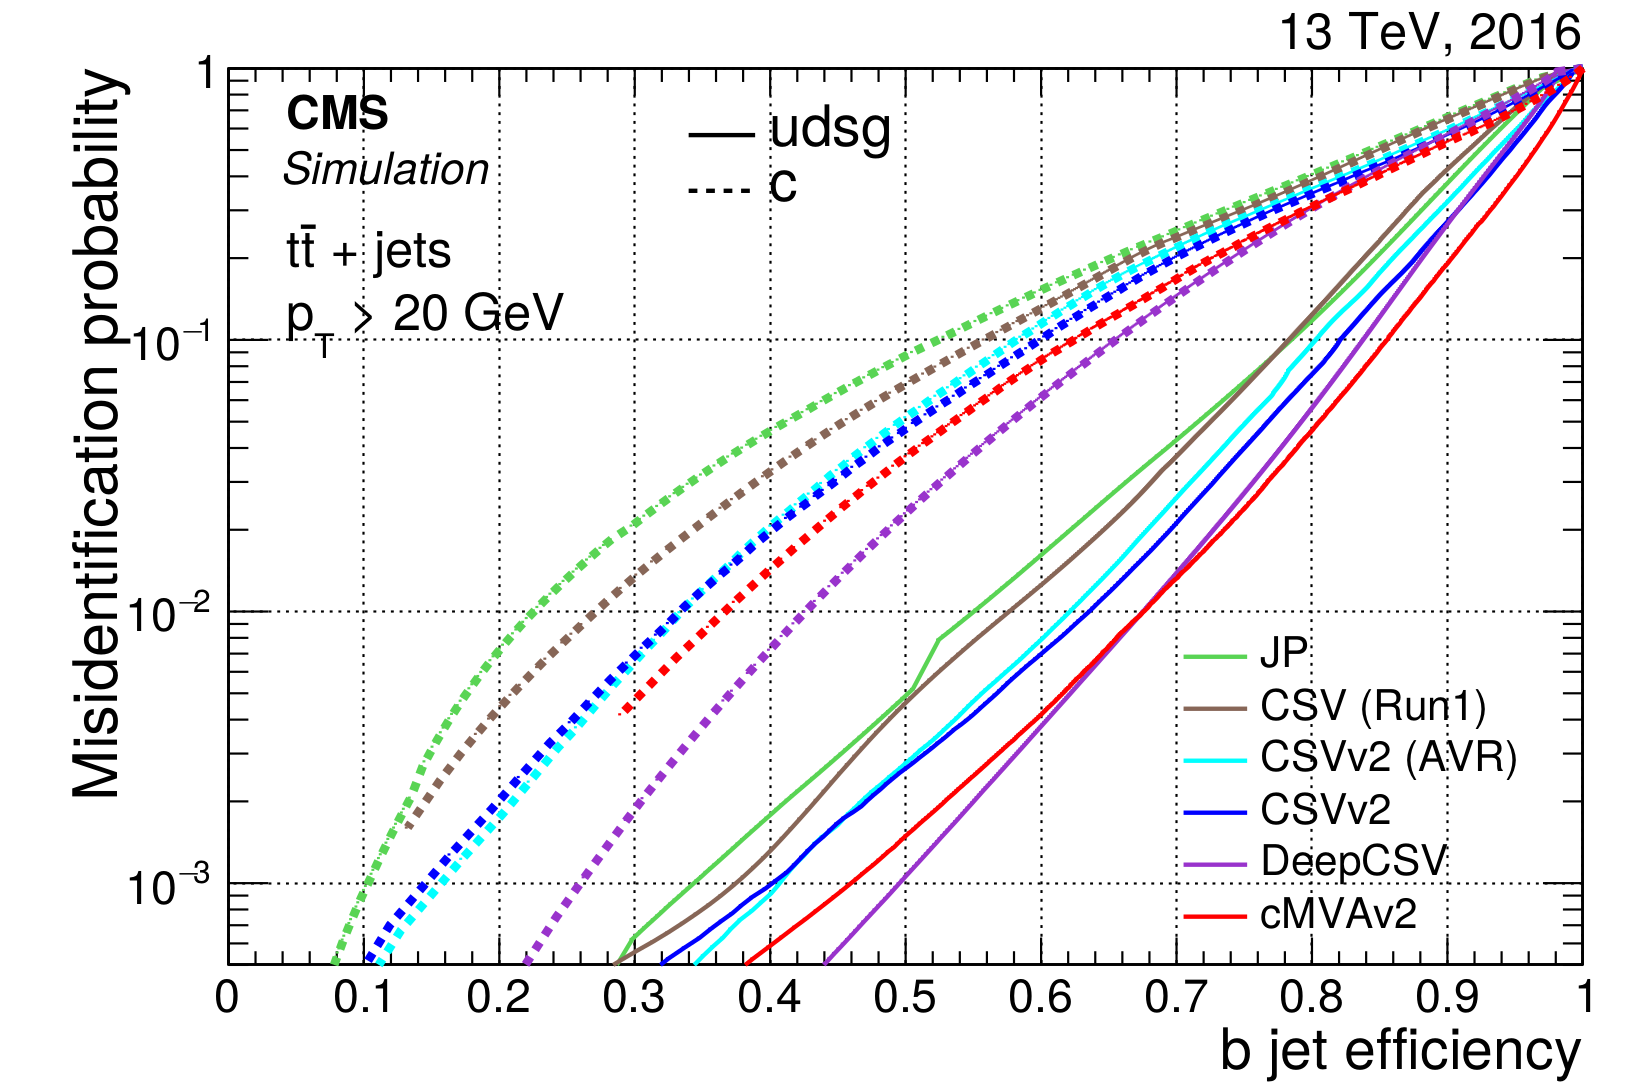
\includegraphics[width=.45\textwidth]{\PhDthesisdir/plots_and_images/from_Sirunyan_heavy_flavor_jets_2018/b_or_mis.png}}

\vspace{\baselineskip}

\subcaptionbox{Probabilité de mauvaise identification en tant que jet de quark~\quarkc\ de jets de gluon ou quarks légers en fonction de l'efficacité d'identification des jets de quark~\quarkc.\label{subfig-chapter-CMS-section-jets_reco-subsec-flavor-c_or_mis}}[.45\textwidth]
{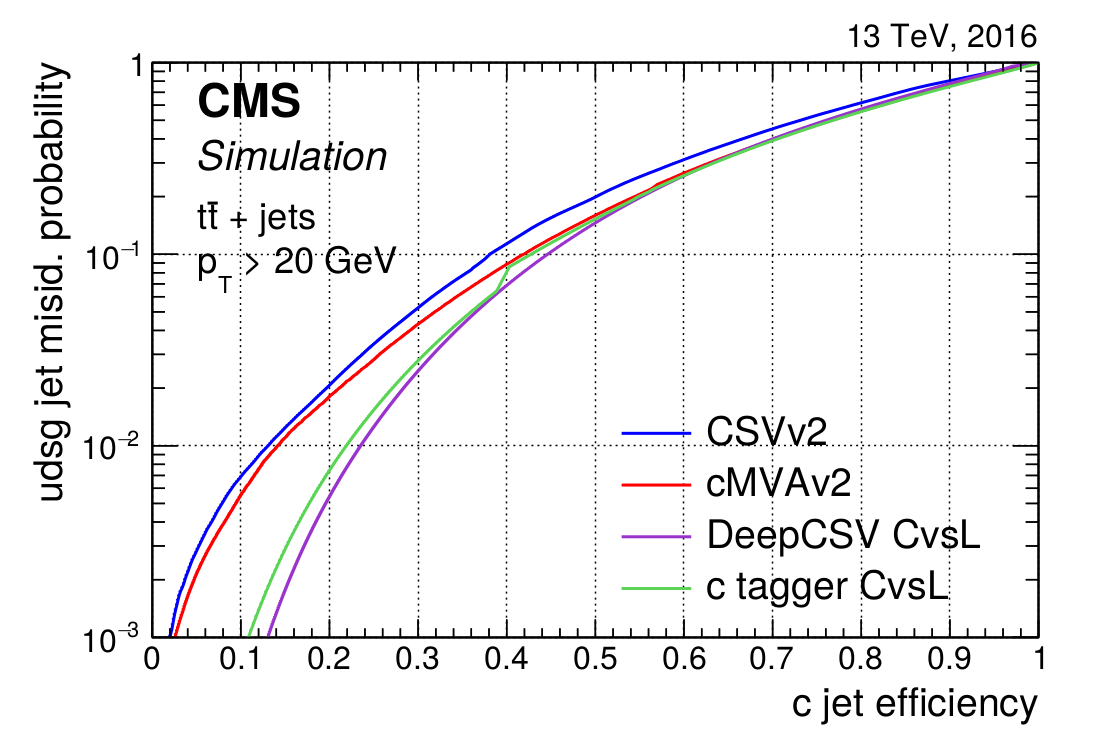
\includegraphics[width=.45\textwidth]{\PhDthesisdir/plots_and_images/from_Sirunyan_heavy_flavor_jets_2018/c_or_mis.png}}
\hfill
\subcaptionbox{Probabilité de mauvaise identification en tant que jet de quark~\quarkb\ de jets de quark~\quarkc en fonction de l'efficacité d'identification des jets de quark~\quarkc.\label{subfig-chapter-CMS-section-jets_reco-subsec-flavor-c_or_b}}[.45\textwidth]
{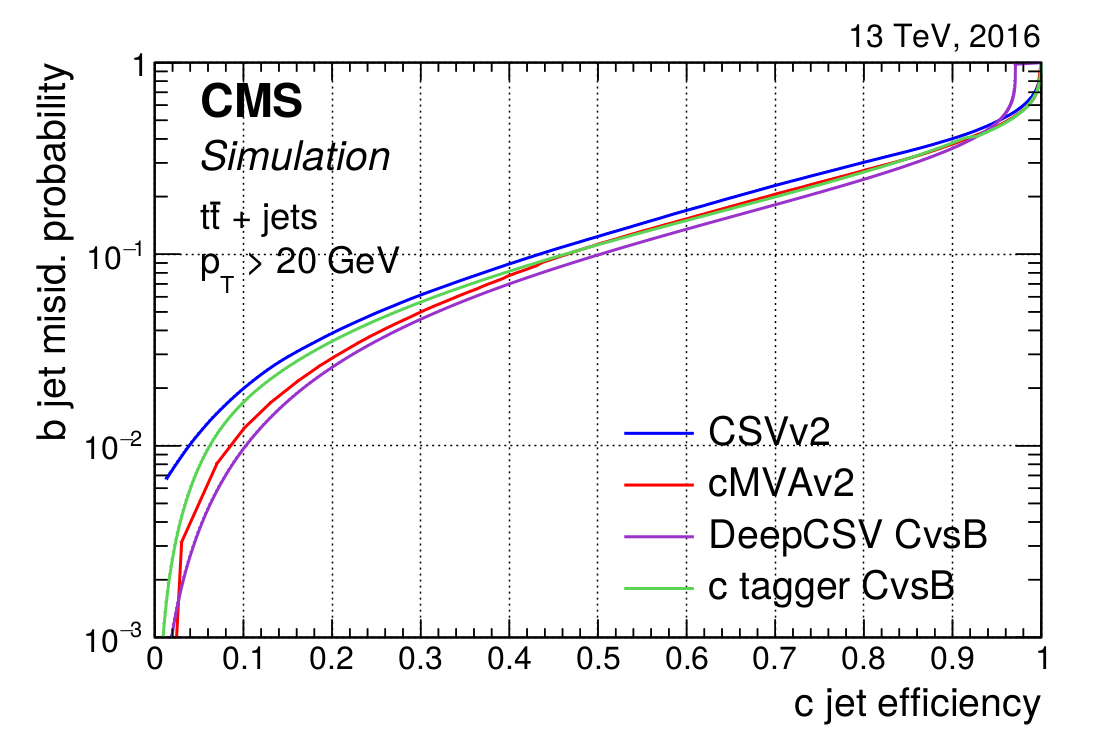
\includegraphics[width=.45\textwidth]{\PhDthesisdir/plots_and_images/from_Sirunyan_heavy_flavor_jets_2018/c_or_b.png}}

\caption[Performances des algorithmes d'identification de la saveur des jets.]{Comparaison des performances des algorithmes d'identification de la saveur des jets~\cite{Sirunyan_heavy_flavor_jets_2018}.}
\label{fig-chapter-CMS-section-jets_reco-subsec-flavor-bc_tag_roc_curves}
\end{figure}
\begin{figure}[p]
\centering
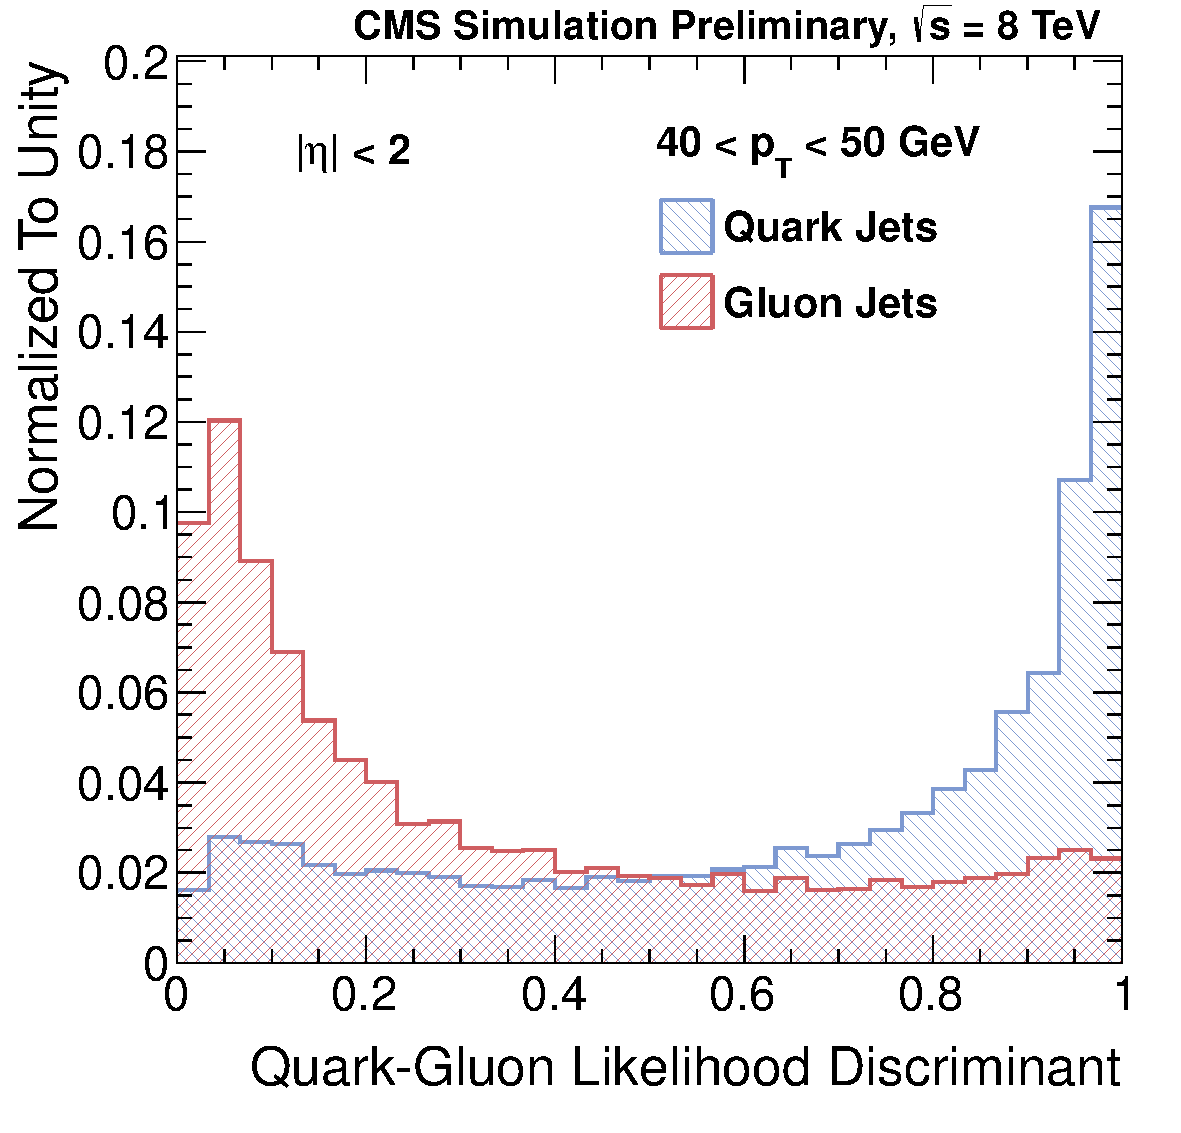
\includegraphics[width=.45\textwidth]{\PhDthesisdir/plots_and_images/from_CMS-PAS-JME-13-002/qgl.pdf}
\caption[Performances de la discrimation quark-gluon pour la saveur des jets.]{Densité de probabilité de la fonction de vraisemblance utilisée pour discriminer les jets issus de gluons de ceux issus de quarks~\cite{CMS-PAS-JME-13-002}. En rouge, pour les jets issus de gluons. En bleu, pour des jets issus de quarks.}
\label{fig-chapter-CMS-section-jets_reco-subsec-flavor-qgl_likelihood}
\end{figure}
%Pour étudier la physique du processus initial, la connaissance du parton à l'origine d'un jet ainsi identifié dans le détecteur est une information de choix.
Il est impossible de connaître avec certitude le parton à l'origine d'un jet,
mais ce dernier possède des propriétés caractéristiques dépendantes du parton, comme exposé dans le chapitre~\refChMSSM.
%Il est impossible de connaître avec certitude cette particule, mais sa nature influe directement sur certaines propriétés des jets, comme exposé dans le chapitre~\refChMSSM.
\par
%Comme exposé dans le chapitre~\refChMSSM,
%les jets présentent des propriétés caractéristiques, selon le parton à leur origine qu'il s'agisse de jets légers (quarks~\quarkd, \quarku\ ou~\quarks), de jets lourds (quarks~\quarkc\ ou~\quarkb) ou de jets issus d'un gluon.
En utilisant ces propriétés, des algorithmes d'identification de la saveur des jets ont été mis au point par la collaboration CMS~\cite{jet_btag_CSV_RunI}.
Les avancées récentes dans le domaine du \emph{Deep Learning}, appliquées à l'identification des jets~\cite{jet_flavor_deep_nn}, ont permis l'amélioration de ces algorithmes.
\DeepCSV~\cite{Sirunyan_heavy_flavor_jets_2018} en est un exemple.
\par Les variables utilisées dans cet algorithme, décrites dans la référence~\cite{Sirunyan_heavy_flavor_jets_2018},
sont traitées par un réseau de neurones profond composé de quatre couches cachées de 100 nœuds connectés les uns aux autres.
Le principe des réseaux de neurones est abordé plus en détails dans le chapitre~\refChML.
Ce réseau a été entraîné à l'aide des librairies
\KERAS~\cite{keras}
et
\TENSORFLOW~\cite{tensorflow}
sur un ensemble d'événements simulés \ttbar, présentant de nombreux jets de quarks~\quarkb, et multijet.
\par Les performances ainsi obtenues pour l'algorithme \DeepCSV\ sont comparées à d'autres algorithmes d'identification de la saveur des jets sur la figure~\ref{fig-chapter-CMS-section-jets_reco-subsec-flavor-bc_tag_roc_curves}.
Les algorithmes \textsc{cMVAv2} et \DeepCSV\ présentent les meilleures performances en termes d'identification des jets de quark~\quarkb\ (\quarkb-\emph{tagging}).
Pour le traitement des jets de quark~\quarkc, l'algorithme \DeepCSV\ propose les meilleures performances.
Dans les analyses présentées dans les chapitres~\refChJERC\ et~\refChHTT, c'est cet algorithme qui est utilisé afin d'identifier les jets issus de quarks~\quarkc\ ou~\quarkb.
\par La discrimination entre jet léger et jet initié par un gluon peut être réalisée à l'aide d'une fonction de vraisemblance~\cite{CMS-PAS-JME-13-002} donnant un score entre 0 et 1 pour chaque jet, correspondant à la probabilité que ce jet soit issu d'un quark. La densité de probabilité de cette fonction, selon qu'il s'agisse de jets initiés par des gluons ou des quarks, est représentée sur la figure~\ref{fig-chapter-CMS-section-jets_reco-subsec-flavor-qgl_likelihood}.
%Sirunyan_heavy_flavor_jets_2018 53
%Cacciari_pu_sub_jet_area_2008 54
%Sarle1994NeuralNA 55
%keras 57
%tensorflow 58
%\emph{The efficiency for the tagging of b jets and the mistagging rate for light-flavour jets has been measured in both data and simulation. The efficiency and mistagging rate of the simulation is corrected through the application of efficiency and mistagging scale factors. The values of these factors and a description of the methods used to determine them can be found in Ref.~\cite{Sirunyan_heavy_flavor_jets_2018}.}